\documentclass[11pt,final,hidelinks]{article}
\usepackage{lmodern}
\usepackage[T1]{fontenc}
\usepackage[english]{babel}
\usepackage[utf8]{inputenc}
\usepackage[activate={true,nocompatibility},final,tracking=true,kerning=true,
    spacing=true,factor=1100,stretch=10,shrink=10]{microtype}
\microtypecontext{spacing=nonfrench}
\usepackage[margin=1in]{geometry}
\usepackage{graphicx}
\graphicspath{{img/}}
\usepackage{caption}
\usepackage{subcaption}
\usepackage{booktabs}
\usepackage{array}
\usepackage{mathtools}
\usepackage{enumitem}
\usepackage{commath}
\usepackage{appendix}
\renewcommand\appendixtocname{Appendices}
\usepackage{amsmath}
\usepackage{amsthm}
\usepackage{amssymb}
%\usepackage[intoc,english]{nomencl}
%\makenomenclature
\usepackage{pgfplots}
\usepackage{tikz}
\usepackage{tikzscale}
\usepackage[square,numbers]{natbib}
\bibliographystyle{plain}
\usepackage{siunitx}
\numberwithin{equation}{section}
\usepackage[hypertexnames=false]{hyperref}
\usepackage{cleveref}

\pgfplotsset{compat=newest}

\usepackage[fancy,section]{alex}

\hypersetup{
    pdftitle={Bernoulli sets: a model for random approximate sets},
    pdfauthor={Alexander Towell},               % author
    pdfsubject={computer science},              % subject of the %document
    pdfkeywords={
        probabilistic data structure,
        abstract data type,
        approximate set,
        bloom filter,
        perfect hash function,
        perfect hash filter},                   % keywords
    colorlinks=true,                            % false: boxed links;
    linkcolor=magenta,
    citecolor=green,                            % color of links to
    filecolor=blue,                             % color of file links
    urlcolor=green                              % color of external
}

\title
{
    Bernoulli sets: a model for random approximate sets
}
\author
{
    Alexander Towell\\
    \texttt{atowell@siue.edu}
}
\date{2026}

\begin{document}
\maketitle
\begin{abstract}
We introduce the \emph{Bernoulli set model}, a probabilistic framework for \emph{random approximate sets}---sets that approximate an objective set with independent, element-wise errors parameterized by false positive and false negative rates.
From two axioms---element-wise independence and conditional independence of block error rates---we derive the binomial distributions of error counts (false positives, false negatives, true positives, true negatives), their asymptotic normal limits, and confidence intervals for the realized error rates.
The model supports higher-order compositions: the $k$-fold composition of approximate identity functions yields a Bernoulli set whose rates are given by the product of binary channel transition matrices.
The framework is formulated as an abstract data type: any implementation satisfying the Bernoulli axioms---including Bloom filters, perfect hash filters, and their compositions---inherits the full theory automatically.
Companion papers develop the compositional set-theoretic algebra, classification measures, and entropy of the model.
\end{abstract}

\microtypesetup{protrusion=false}
\tableofcontents
\microtypesetup{protrusion=true}

%%%%%%%%%%%%%%%%%%%%%%%%%%%%%%%%
% Introduction
%%%%%%%%%%%%%%%%%%%%%%%%%%%%%%%%

\section{Introduction}

Many computational systems rely on \emph{approximate set representations}---data structures whose membership queries may err, returning false positives or false negatives with known rates.
Bloom filters~\cite{bf}, perfect hash filters~\cite{phf}, and related probabilistic data structures achieve dramatic space savings by tolerating such errors, and individual structures are well understood.
However, practical systems rarely use a single approximate set in isolation.
Encrypted search indexes, database query planners, and distributed systems routinely compose approximate sets through union, intersection, complement, and difference, and the resulting error behavior has traditionally been analyzed on a case-by-case basis.

\paragraph{The gap.}
The existing literature lacks a \emph{compositional algebra} for approximate sets: a framework in which the error rates of any set-theoretic expression are mechanically computable from the error rates of its operands.
Without such a framework, each new combination of approximate sets requires a bespoke analysis, and higher-order compositions---approximate sets of approximate sets---remain largely uncharacterized.

\paragraph{Contribution.}
We introduce the \emph{Bernoulli set model}, a probabilistic framework for \emph{random approximate sets} built on two axioms: element-wise independence of errors and conditional independence of block error rates.
From these axioms we derive:
\begin{enumerate}[nosep]
    \item the binomial distributions of error counts (false positives, false negatives, true positives, true negatives) and their asymptotic normal limits,
    \item the higher-order composition theorem: the $k$-fold composition of approximate identity functions yields a Bernoulli set whose rates are given by the product of binary channel transition matrices, and
    \item confidence intervals for the realized false positive and true positive rates.
\end{enumerate}
The framework is formulated as an abstract data type: any implementation whose membership queries satisfy the Bernoulli axioms---including Bloom filters, perfect hash filters, and their compositions---inherits the full theory automatically.

\paragraph{Related work.}
The original Bloom filter~\cite{bf} introduced approximate set membership with one-sided error.
Subsequent work has produced a rich family of probabilistic data structures---including cuckoo filters~\cite{cuckooFilter}, quotient filters~\cite{quotientFilter}, xor filters~\cite{xorFilter}, and ribbon filters~\cite{ribbonFilter}---surveyed by Broder and Mitzenmacher~\cite{broderMitzenmacher}, with improved space efficiency or additional functionality.
Bose et al.~\cite{boseBloom} give tight bounds on the Bloom filter false positive rate, Kirsch and Mitzenmacher~\cite{kirschMitzenmacher} show that two hash functions suffice, and Carter and Wegman~\cite{carterWegman} provide the universal hash families underlying many implementations.
Related probabilistic summaries such as the count-min sketch~\cite{countMinSketch} trade exact answers for space efficiency in the streaming setting.
However, analyses typically treat each structure in isolation, deriving error rates for a single filter rather than for compositions of filters.
General probabilistic methods for randomized algorithms~\cite{mitzenmacherUpfal} provide the analytical toolkit (concentration inequalities, entropy bounds) but do not address the compositional structure of approximate sets.
Our framework complements these lines of work by providing an algebraic layer that sits above any particular implementation; the interval arithmetic extension for uncertain rate parameters is developed in~\cite{bernoulliComposition}.

\paragraph{Companion papers.}
The set-theoretic composition of Bernoulli sets---closed-form error rates for complement, union, intersection, and set difference, monoidal structure, relational predicates, and interval arithmetic---is developed in a companion paper~\cite{bernoulliComposition}.
The probability distributions of binary classification measures (precision, recall, accuracy, etc.) induced by the Bernoulli model are derived in~\cite{bernoulliMeasures}.
The joint entropy of error counts and the information-theoretic space complexity of approximate sets are developed in~\cite{bernoulliEntropy}.

\paragraph{Organization.}
\Cref{sec:setalgebra} reviews the algebra of sets.
\Cref{sec:bernoulli_model} introduces the Bernoulli set model and its axioms, including the higher-order composition theorem.
\Cref{sec:characteristics} derives the binomial distributions of error counts and their asymptotic normal limits.

%%%%%%%%%%%%%%%%%%%%%%%%%%%%%%%
% Algebra of sets
%%%%%%%%%%%%%%%%%%%%%%%%%%%%%%%

\section{Algebra of sets} 
\label{sec:setalgebra}
A \emph{set} is an unordered collection of distinct elements.
If we know the elements in a set, we may denote the set by these elements, e.g., $\{a,c,b\}$ denotes a set whose members are exactly $a$, $b$, and $c$.

Two sets of particular importance are the empty set, denoted by $\emptyset$, which has no members, and the \emph{universal set}, in which every element of interest is a member.

The \emph{cardinality} of a finite set $A$ is the number of elements in $A$, denoted by $|A|$.
A \emph{countably infinite set} is one that can be put into bijection with $\mathbb{N} = \{1,2,\ldots\}$.
We assume familiarity with standard set-theoretic notation (ordered pairs, Cartesian products, relations, functions); see Feller~\cite{feller} for background.

The \emph{power set} of $A$, denoted by $\mathcal{P}(A)$, is the set of all subsets of $A$.
The \emph{indicator function} of $A$ with respect to a universal set $X$ is
\begin{equation}
	\mathbf{1}_A : X \to \{0,1\}, \quad
	\mathbf{1}_A(x) =
	\begin{cases}
		1 & \text{if $x \in A$},\\
		0 & \text{if $x \notin A$}.
	\end{cases}
\end{equation}
The standard set operations---\emph{union} $A \cup B = \{x : x \in A \lor x \in B\}$, \emph{intersection} $A \cap B = \{x : x \in A \land x \in B\}$, and \emph{complement} $A^c = \{x \in X : x \notin A\}$---are used throughout.
Sets $A$ and $B$ are \emph{disjoint} if $A \cap B = \emptyset$.

\subsection{Approximate sets}
\label{sec:asets}
Given an objective set $A$, any element that is a member of $A$ is denoted a \emph{positive} (of $A$) and otherwise the element is denoted a \emph{negative}.
We write $\hat{A}$ for an arbitrary approximation of $A$; in \cref{sec:bernoulli_model}, this will be refined to the Bernoulli set $\tilde{A}$, which satisfies additional axioms.
Suppose $\hat{A}$ is used as an \emph{approximation} of $A$.
If the \emph{only} information we have about $A$ is given by $\hat{A}$, then we may perform membership tests on $\hat{A}$ to make \emph{predictions} or \emph{estimations} about $A$.

There are two ways a binary prediction can be false.
\begin{enumerate}
	\item A \emph{false positive} occurs if a negative of the objective set is predicted to be a positive. False positives are also known as \emph{type I errors}.
	The complement of false positives are \emph{true negatives}.
	\item A \emph{false negative} occurs if a positive of the objective set is predicted to be a negative. False negatives are also known as \emph{type II errors}.
	The complement of false negatives are \emph{true positives}.
\end{enumerate} 

If we denote the set of false positives by $FP$, true positives by $TP$, false negatives by $FN$, and true negatives by $TN$, then the objective set $A = FN \cup TP$ and the approximate set $\hat{A} = TP \cup FP$.
See \cref{fig:ex_approx_set} for an illustration.
\begin{figure}[ht]
	\centering
	\def\svgwidth{\columnwidth/4}
	\input{img/aset_fp_fn.tex}
	\caption{An approximate set $\hat{A}$ of an objective set $A$}
	\label{fig:ex_approx_set}
\end{figure}

If we only have access to the approximation $\hat{A}$, we do not have the ability to partition the universe into the disjoint sets $FP$, $TP$, $FN$, and $TN$ as demonstrated in \cref{fig:ex_approx_set}.
However, we can quantify the degree of \emph{uncertainty} about the elements that it predicts to be positive or negative.
The false positive and true negative rates are given by the following.
\begin{definition}
	\label{def:fprate}
	The \emph{false positive rate} is the proportion of predictions that are \emph{false positives} as given by
	\begin{equation}
	\hat{\alpha} = \frac{|FP|}{|FP| + |TN|}
	\end{equation}
	and the \emph{true negative rate} is given by $\hat{\tnrate} = 1 - \hat{\alpha}$.
\end{definition}
The true positive and false negative rates are given by the following.
\begin{definition}
	The \emph{true positive rate} is the proportion of predictions that are \emph{true positives} as given by
	\begin{equation}
	\hat{\tprate} = \frac{|TP|}{|TP| + |FN|}
	\end{equation}
	and the \emph{false negative rate} is given by $\hat{\beta} = 1 - \hat{\tprate}$.
\end{definition}

The \emph{probabilities} of the four possible predictive outcomes are given by 
\cref{tbl:contingency_table}.
\begin{table}[ht]
	\centering
	\begin{tabular}{@{} l l l @{}}
		\toprule
		& \textbf{positive} & \textbf{negative}\\
		\midrule
		\textbf{predict positive} & $\hat{\tprate}=1-\hat{\beta}$ & 
		$\hat{\alpha}=1-\hat{\tnrate}$\\
		\textbf{predict negative} & $\hat{\beta}=1-\hat{\tprate}$ & 
		$\hat{\tnrate}=1-\hat{\alpha}$\\
		\bottomrule
	\end{tabular}
	\caption{The $2 \times 2$ contingency table of outcomes for approximate sets.}
	\label{tbl:contingency_table}        
\end{table}

%%%%%%%%%%%%%%%%%%%%%%%%%%%%%%%%%
% Bernoulli model
%%%%%%%%%%%%%%%%%%%%%%%%%%%%%%%%%

\section{Bernoulli set model}
\label{sec:bernoulli_model}
In the \emph{Bernoulli} set model, we describe the statistical properties of processes that \emph{generate} approximations of a certain kind that model many existing processes and generalizes to higher-order approximations under algebraic composition.

In what follows, we specify the axioms of the Bernoulli set model.

Theoretically, a process that generates approximations could exhibit correlations of any sort, but Bernoulli sets are constrained by the following axiom.
\begin{axiom}[Element-wise independence]
\label{asm:element_indep}
For all distinct $x, y \in U$, the error events at $x$ and $y$ are mutually independent:
\begin{equation}
P(\mathbf{1}_{\tilde{A}}(x) \neq \mathbf{1}_{A}(x) \mid \mathbf{1}_{\tilde{A}}(y) \neq \mathbf{1}_{A}(y)) =
	P(\mathbf{1}_{\tilde{A}}(x) \neq \mathbf{1}_{A}(x)).
\end{equation}
More generally, the family $\{\mathbf{1}_{\tilde{A}}(x) : x \in U\}$ is mutually independent given the objective set $A$ and the error rates.
Furthermore, within each partition block $B_i$ (\cref{def:model_order}), the error indicators $\{\mathbf{1}_{\tilde{A}}(x) : x \in B_i\}$ are identically distributed.
\end{axiom}

The complexity in the Bernoulli set model stems from the fact that different subsets of the universal set may exhibit different error rates.
Suppose the objective set $R \in 2^U$ induces a partition $\{B_1, \ldots, B_n\}$ of $U$ such that elements within each block $B_i$ share a common error rate $\alpha_i$.
\begin{definition}[Model order]
\label{def:model_order}
The \emph{order} of a Bernoulli set model is the number of partition blocks $n$.
A zeroth-order model ($n = 0$) is the degenerate case: no partition blocks and no errors (the exact set).
A first-order model ($n = 1$) assigns a single error rate to all elements (symmetric channel).
A second-order model ($n = 2$) distinguishes positives from negatives with rates $\tprate$ and $\fprate$ respectively.
In general, an $n$-th order model partitions $U$ into $n$ blocks, each with its own error rate; the maximum order is $|U|$.
\end{definition}
In the second-order (positive-negative) model, $n = 2$: the partition is $\{R, R^c\}$ with block response rates $\alpha_1 = \beta$ (response rate on positives, i.e., true positive rate) and $\alpha_2 = \alpha$ (response rate on negatives, i.e., false positive rate).
\begin{axiom}[Conditional independence of block error rates]
\label{asm:fpr_fnr_r_indep}
Given the objective set $R$, the random error rates $\alpha_1, \ldots, \alpha_n$ for the respective partition blocks $B_1, \ldots, B_n$ are mutually independent.
\end{axiom}
For instance, in the second-order model, the random false positive rate $\alpha$ and the random true positive rate $\beta$ are conditionally independent given $R$.

\begin{remark}[Relation to the binary symmetric channel]
\label{rem:bsc}
At the per-element level, the Bernoulli set model is a collection of independent binary symmetric channels~\cite{shannonBSC}; equivalently, each element undergoes Warner's randomized response~\cite{warner1965}. For each $x \in U$, the indicator $\mathbf{1}_{\tilde{A}}(x)$ is the output of a BSC with crossover probability $\fprate$ (if $x \notin A$) or $\fnrate$ (if $x \in A$).
The novelty of the present framework is not the per-element channel model, which is classical, but the \emph{set-level} compositional algebra: the derivation of error rates for union, intersection, complement, and their higher-order compositions over collections of such channels.
\end{remark}

\begin{remark}[Axiom economy]
\label{rem:axiom_economy}
Most results in this paper---the distributions of all binary classification measures (\cref{sec:characteristics}), the set-operation error rates and monoidal structure (\cref{sec:set_theory}), and the relational probabilities (\cref{sec:relational})---follow from \cref{asm:element_indep} alone.
\Cref{asm:fpr_fnr_r_indep} is needed only when the objective set $R$ is itself uncertain, in which case it permits the factorization of the joint distribution of $\tilde{R}$ and $R$ (\cref{sec:prob_model}) and the entropy decomposition (\cref{sec:entropy}).
\end{remark}

There are two natural \emph{statistics} of the Bernoulli set model, the random false positive and true positive rates conditioned on $R = A$.
They are respectively defined by
\begin{equation}
\label{def:sample_fprate}
	\alpha = \frac{1}{|A^c|} \sum_{x \in A^c} \mathbf{1}_{\tilde{A}}(x)
\end{equation}
and
\begin{equation}
\label{def:sample_tprate}
	\beta = \frac{1}{|A|} \sum_{x \in A} \mathbf{1}_{\tilde{A}}(x).
\end{equation}
\begin{proposition}
\label{prop:element_rates}
By \cref{asm:element_indep}, for any single element $x \notin A$,
$\Prob{\mathbf{1}_{\tilde{A}}(x) = 1} = \fprate$, and for $x \in A$,
$\Prob{\mathbf{1}_{\tilde{A}}(x) = 1} = \tprate$.
The expected sample rates satisfy $E[\alpha] = \fprate$ and $E[\beta] = \tprate$.
\end{proposition}



We denote the second-order random approximate set generative model by $\tilde{R}$, with random false positive rate $\alpha$ and random true positive rate $\beta$ conditioned on the objective set $R$.
The conditional distribution of $\tilde{R}$ given $R = X$ is denoted by $\tilde{X}$.
When the rates are degenerate, the model reduces to a deterministic outcome, e.g., $\tilde{A}$ given $\alpha = 0$ and $\beta = 1$ places all probability mass on $A$.

We parameterize $\tilde{X}$ by its expected false positive rate $\fprate$ and expected true positive rate $\tprate$, writing
\begin{equation}
\tilde{X}[\fprate][\tprate].
\end{equation}
We define the complementary rates $\fnrate = 1-\tprate$ (FNR) and $\tnrate = 1-\fprate$ (TNR) as shorthands that appear naturally in derived expressions.
Special cases with only one type of error specified are written $\tilde{X}[\fprate][-]$ and $\tilde{X}[+][\tprate]$.

Random \emph{positive} and \emph{negative} approximate sets are special cases respectively given by the following definitions.
\begin{definition}
\label{def:pos_approx_set}
A random approximate set $\tilde{A}[0][+]$ is a random \emph{positive} approximate set denoted by $\tilde{A}_+$.
\end{definition}
\begin{definition}
\label{def:neg_approx_set}
A random approximate set $\tilde{A}[-][0]$ is a random \emph{negative} approximate set denoted by $\tilde{A}_-$.
\end{definition}
By these definitions, every realization of $\tilde{A}_+$ and $\tilde{A}_-$ are respectively \emph{supersets} or \emph{subsets} of $A$.
The complement of a random positive (negative) approximate set is a random negative (positive) approximate set.

By \cref{asm:fpr_fnr_r_indep} and by the axioms of probability,
\begin{equation}
f(\tilde{X}, \alpha, \beta) =
f(\tilde{X} | \alpha, \beta)
f(\alpha | R) f(\beta | R).
\end{equation}

Every statistical property of the second-order random approximate set model is entailed by \cref{def:sample_fprate,def:sample_tprate}.
Furthermore, these assumptions generally hold in practice, e.g., the Bloom filter~\cite{bf} and Perfect hash filter~\cite{phf} are two separate implementations of the random positive approximate set in which these assumptions hold.

\subsection{Abstract data type}
\label{sec:adt}
A data type $T$ that overloads the membership predicate $\SetContains : U \times T \to \{0,1\}$ and has a value constructor $\ctor{\fprate}{\tprate} : 2^U \to T$ \emph{models} the Bernoulli set abstract data type if \cref{def:sample_fprate,def:sample_tprate} are satisfied, i.e.,
\begin{equation}
	\Prob{\SetContains[x][\ctor{\fprate}{\tprate}(A)] | \SetNotContains[x][A]} = \fprate
\end{equation}
and
\begin{equation}
	\Prob{\SetContains[x][\ctor{\fprate}{\tprate}(A)] | \SetContains[x][A]} = \tprate.
\end{equation}
Two data types that model Bernoulli sets with the same expected error rates are interchangeable in the frequentist sense: at the limit of repeated independent runs, they produce the same distribution over outcomes.

Suppose the second-order random approximate sets are over the universal set $U$.
Compositions of second-order random approximate sets over the Boolean algebra $(2^U,\cup,\SetIntersection,\SetComplement,\EmptySet,U)$, or random approximate sets of random approximate sets, are not closed over the \emph{second-order} model.
These compositions are addressed in the higher-order model below.

\subsection{Higher-order models and composition}
\label{sec:higher_order_model}

We compose \emph{random approximate sets} over the Boolean algebra $(\Sigma,\SetUnion,\SetIntersection,\SetComplement,\EmptySet,\Set{U})$, where $\Sigma \subseteq \PS{\Set{U}}$ because a deterministic implementation may not reach every element of $\PS{\Set{U}}$.
As a result, to satisfy the identity and complementation axioms required by Boolean algebras, we make $\EmptySet$ and $\Set{U}$ available in the model as special cases.
\begin{remark}
	Alternatively, these axioms may be satisfied by making the empty set and the universal set \emph{degenerate} cases, i.e., $\Prob{\ASet{\EmptySet} = \EmptySet} = 1$ and $\Prob{\ASet{U} = \Set{U}} = 1$.
\end{remark}

Furthermore, we may replace any of the operators in the Boolean algebra with \emph{random approximations} that model the noisy or rate-distorted channel previously described, i.e., these operators may themselves be constructors for random approximate sets, e.g., $\Set{A} \, \AT{\SetUnion}[\fprate][\tprate] \, \Set{B} \sim \AT{(\SetUnion[\Set{A}][\Set{B}])}[\tprate][\fprate]$ where $\AT{\SetUnion}[\fprate][\tprate]$ maps negatives to positives with probability $\fprate$ and maps positives to negatives with probability $\tprate$.

A natural mapping is provided by the \emph{identity} function $\Fun{id} \colon \PS{\Set{X}} \to \PS{\Set{X}}$, which is defined as
\begin{equation}
\Fun{id}(\Set{A}) \coloneqq \Set{A}\,.
\end{equation}
However, suppose we only have an \emph{approximation} of the identity function, denoted by $\APFun{id}[\fprate][\tprate]$, such that $\APFun{id}[\fprate][\tprate](\Set{A}) \sim \ASet{A}[\fprate][\tprate]$.
Then $\APFun{id}[\fprate][\tprate]$ generates sets consistent with the random approximate set model.

If we compose random approximate sets, then we have \emph{higher-order} random approximate sets.
\begin{theorem}
\label{thm:composition_rates}
	The composition of random approximate identity functions $\APFun{id}[\fprate][\tprate] \circ \APFun{id}[\fprate'][\tprate']$ generates random approximate sets with a true positive rate $\tprate' \tprate + \fnrate' \fprate$ and false positive rate $\fprate' \tprate + \tnrate' \fprate$.
\end{theorem}
\begin{proof}
	Let $x \in A$. In the inner approximation $\APFun{id}[\fprate'][\tprate']$, element $x$ tests positive with probability $\tprate'$ and negative with probability $\fnrate' = 1 - \tprate'$.
	In the outer approximation $\APFun{id}[\fprate][\tprate]$, a positive is retained with probability $\tprate$ and a negative is promoted to positive with probability $\fprate$.
	By the law of total probability, the composed true positive rate is
	$\tprate' \cdot \tprate + \fnrate' \cdot \fprate$.
	Similarly, let $x \notin A$. In the inner approximation, $x$ tests positive with probability $\fprate'$ and negative with probability $\tnrate' = 1 - \fprate'$.
	The composed false positive rate is
	$\fprate' \cdot \tprate + \tnrate' \cdot \fprate$.
\end{proof}

\begin{definition}
	The \emph{iterated} function $\Fun{f}^k$ is defined as $k$ compositions of $\Fun{f}$ where $\Fun{f}^0$ denotes the (non-random) \emph{identity} function.
\end{definition}
The composition $\left(\APFun{id}[\fprate][\tprate]\right)^k$ generates $k$-fold compositions of random approximate sets where the \emph{zero-th} order random approximation is the identity, i.e., $\left(\APFun{id}\right)^0 = \Fun{id}$.

The function being approximated may take other forms, like \emph{set-complementation} or \emph{set-union}, e.g.,
let $\SetUnion \colon \PS{\Set{X}} \times \PS{\Set{X}} \to \PS{\Set{X}}$ be approximated by $\APFun{\SetUnion}[\fprate][\tprate] \colon \PS{\Set{X}} \times \PS{\Set{X}} \to \PS{\Set{X}}$.
Then, $\Set{A} \APFun{\SetUnion}[\fprate][\tprate] \Set{B}$ is a random approximate set of $\SetUnion[\Set{A}][\Set{B}]$ as before.
However, $\APFun{\SetUnion}[\fprate'][\tprate'] \circ \APFun{id}[\fprate][\tprate]$ generates two-fold compositions of random approximate sets.

\begin{theorem}
\label{thm:twofold_composition}
	Given a random approximate set $\ASet{A}[\fprate_1][\tprate_1]$, a random approximation of $\ASet{A}[\fprate_1][\tprate_1]$ with a false positive rate $\fprate_2$ and true positive rate $\tprate_2$ is a \emph{two-fold composition} approximating $\Set{A}$ with a false positive rate $\fprate = \fprate_1 \tprate_2 + \tnrate_1 \fprate_2$ and true positive rate $\tprate = \tprate_1 \tprate_2 + \fnrate_1 \fprate_2$, denoted by $\Set{A}^{\sigma^2}(\tprate,\fprate)$.

	This result may be recursively applied to derive arbitrary $k$-fold compositions as given by
	\begin{equation}
		\Set{A}^{\sigma^k} = \left(\Set{A}^{\sigma^{k-1}}\right)^{\sigma}
	\end{equation}
	where the \emph{zero-th} order $\Set{A}^{\sigma^0} = \Set{A}$.
\end{theorem}
\begin{proof}
The result follows by applying \cref{thm:composition_rates} with inner
rates $(\fprate_1, \tprate_1)$ and outer rates $(\fprate_2, \tprate_2)$.
The recursive formula holds by induction: the base case $k = 0$ is the
exact identity, and the inductive step applies \cref{thm:composition_rates}
to the $k$-th order rates as inner parameters.
\end{proof}

\begin{figure}[ht]
\centering
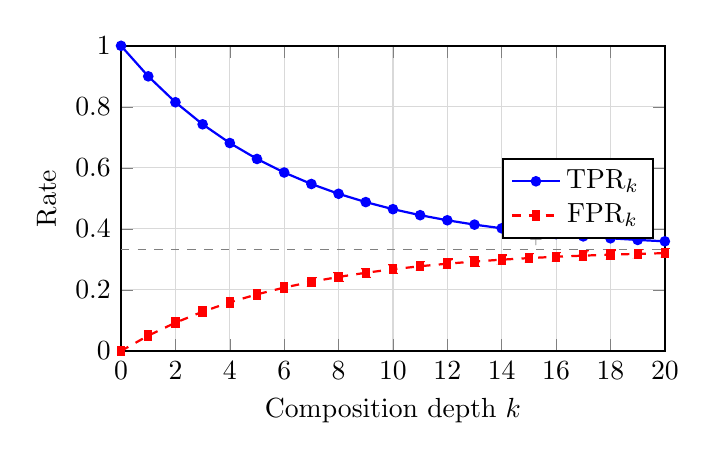
\begin{tikzpicture}
\begin{axis}[
	width=0.7\textwidth,
	height=0.45\textwidth,
	xlabel={Composition depth $k$},
	ylabel={Rate},
	xmin=0, xmax=20,
	ymin=0, ymax=1,
	legend style={at={(0.98,0.5)}, anchor=east},
	ymajorgrids, xmajorgrids,
	major grid style={gray!30},
	thick,
	xtick={0,2,...,20},
]
\addplot[blue, solid, mark=*, mark size=1.5pt] coordinates {
	(0,1.00000000) (1,0.90000000) (2,0.81500000)
	(3,0.74275000) (4,0.68133750) (5,0.62913688)
	(6,0.58476634) (7,0.54705139) (8,0.51499368)
	(9,0.48774463) (10,0.46458294) (11,0.44489550)
	(12,0.42816117) (13,0.41393700) (14,0.40184645)
	(15,0.39156948) (16,0.38283406) (17,0.37540895)
	(18,0.36909761) (19,0.36373297) (20,0.35917302)
};
\addlegendentry{TPR$_k$}
\addplot[red, dashed, mark=square*, mark size=1.5pt] coordinates {
	(0,0.00000000) (1,0.05000000) (2,0.09250000)
	(3,0.12862500) (4,0.15933125) (5,0.18543156)
	(6,0.20761683) (7,0.22647430) (8,0.24250316)
	(9,0.25612768) (10,0.26770853) (11,0.27755225)
	(12,0.28591941) (13,0.29303150) (14,0.29907678)
	(15,0.30421526) (16,0.30858297) (17,0.31229553)
	(18,0.31545120) (19,0.31813352) (20,0.32041349)
};
\addlegendentry{FPR$_k$}
\addplot[gray, thin, dashed, forget plot, domain=0:20] {1/3};
\node[anchor=west, gray] at (axis cs:14.5,0.37) {$\scriptstyle\frac{\fprate}{\fprate+\fnrate}$};
\end{axis}
\end{tikzpicture}
\caption{True positive rate and false positive rate under $k$-fold
composition of the approximate identity
$\APFun{id}[\fprate][\tprate]$ with $\fprate = 0.05$ and $\tprate = 0.90$.
Both rates converge to the stationary point
$\fprate/(\fprate + \fnrate) = 1/3$, where $\fnrate = 1 - \tprate$.
At high $k$, the approximation degrades toward a coin flip weighted by the
channel's stationary distribution.}
\label{fig:kfold_composition}
\end{figure}

In an \emph{algebra of sets} $(\PS{\Set{U}}, \SetIntersection, \SetUnion, \SetComplement, \Set{U}, \EmptySet)$, we may compose sets to form new sets.
When these sets model \emph{random approximate sets}, then their compositions model \emph{higher-order} random approximate sets, e.g.,
$\SetUnion[\ASet{A}[\fprate_1][\tprate_1]][\ASet{B}[\fprate_2][\tprate_2]]$
models a higher-order random approximate set which does not obey the second-order model; rather, it partitions the negative set such that each partition may have a different false positive rate and similarly for the positive set.

This contrasts with $\AT{\left(\SetUnion[\Set{A}][\Set{B}]\right)}[\fprate][\tprate]$, in which the false positive rate for the negative elements are uniformly distributed and likewise for the positive elements.
We call these random approximate sets \emph{second-order} approximations.
For completeness, the \emph{zeroth-order} are the objective sets, e.g., the zeroth-order approximation of $\SetUnion[\Set{A}][\Set{B}]$ is $\SetUnion[\Set{A}][\Set{B}]$.
The complexity of the probabilistic model increases as the order increases.

\subsection{Probability space}
\label{sec:prob_model}
The sample space is $\Omega = 2^U$, and the probability space is $(\Omega, \PS{\Omega}, P)$.
By \cref{asm:element_indep}, the conditional distribution of $\tilde{A}$ given the objective set $A$ factorizes element-wise:
\begin{equation}
    \Prob{\tilde{A} = S \Given A} = \prod_{x \in U} \Prob{\mathbf{1}_{\tilde{A}}(x) = \mathbf{1}_S(x) \Given \mathbf{1}_A(x)},
\end{equation}
where each factor equals $\tprate$ or $\fprate$ (if the element tests positive) or $\fnrate$ or $\tnrate$ (if it tests negative), depending on whether $x \in A$.

\begin{remark}[Latent and observed sets]
\label{rem:latent_observed}
The Bernoulli set model induces a duality between the \emph{latent} (objective) set $A$
and the \emph{observed} (approximate) set $\tilde{A}$.
Given the error model, the observed set constrains the possible latent sets.
For instance, if $\tilde{A}$ is a positive approximate set ($\fnrate = 0$),
then $A \subseteq \tilde{A}$: every element of $\tilde{A}$ is either a true positive
or a false positive, so the latent set must be a subset of the observed set.
Conversely, elements absent from $\tilde{A}$ are certainly absent from $A$.
\end{remark}


Consider the following example.
\begin{example}[Boolean universe]
\label{ex:boolean_universe}
	Let the universal set be $U = \{\top, \bot\}$ (the Boolean values \emph{true} and \emph{false}) and let the objective set be $A = \{\top\}$.
	A Bernoulli set $\tilde{A}^\fprate_\tprate$ over this universe has four possible outcomes, enumerated by the probability mass function
	\begin{equation}
	p_{\tilde{A}^\fprate_\tprate}(\Set{X}) =
	\begin{cases}
	\fnrate \cdot \tnrate & \Set{X} = \EmptySet,\\
	\fnrate \cdot \fprate & \Set{X} = \{\bot\},\\
	\tprate \cdot \tnrate & \Set{X} = \{\top\},\\
	\tprate \cdot \fprate & \Set{X} = \{\top, \bot\}.
	\end{cases}
	\end{equation}
	The outcome $\Set{X} = \{\top, \bot\}$ means both a true positive ($\top \in \tilde{A}$) and a false positive ($\bot \in \tilde{A}$) occurred.
	The outcome $\Set{X} = \{\bot\}$ means a false positive and a false negative occurred simultaneously.
	In the positive approximate set ($\fnrate = 0$), only $\Set{X} \in \{\{\top\}, \{\top, \bot\}\}$ are reachable, so $A \subseteq \tilde{A}$ with certainty.
\end{example}

\begin{remark}[Membership tests as Bernoulli Booleans]
\label{rem:membership_boolean}
For a Bernoulli set over an arbitrary universe $U$, the membership test $x \in \tilde{A}$ returns a Boolean value that is itself a Bernoulli approximation of the latent answer $x \in A$.
Consider a positive approximate set such as a Bloom filter, where $\fnrate = 0$.
If we query an element $x$ and observe $x \in \tilde{A}_+$, the result may be a false positive: $x$ might not belong to the latent set $A$.
If we observe $x \notin \tilde{A}_+$, the result is certainly a true negative: $x \notin A$.
Thus each membership query projects the set-level Bernoulli model onto the Boolean universe of \cref{ex:boolean_universe}, yielding a single Bernoulli Boolean whose error structure is inherited from the underlying set.
This pattern extends beyond data structures.
The Miller--Rabin primality test returns ``composite'' (certainly correct) or ``probably prime'' (false positive with probability at most $1/4$ per round), making its output a positive Bernoulli Boolean: the latent answer is $\{\text{prime}\}$ or $\{\text{composite}\}$, and the observed answer is a one-sided approximation with $\fnrate = 0$ and $\fprate \leq 1/4$.
More generally, any randomized decision procedure with one-sided error produces Bernoulli Booleans.
\end{remark}

%%%%%%%%%%%%%%%%%%%%%%%%%%%%%%%%%

%%%%%%%%%%%%%%%%%%%%%%%%%%%%%%%%%
% Distributions of error counts
%%%%%%%%%%%%%%%%%%%%%%%%%%%%%%%%%%%
\section{Distributions of error counts}
\label{sec:characteristics}
The error rate on some identically distributed subset is an \emph{expectation}.
However, some \emph{error measures} span multiple subsets, such as positives and negatives.
Any such error measure may be modeled as a \emph{Bernoulli mixture}.

We are typically interested in the error rates of \emph{special} subsets.
For example, if we have a universal set $\Set{X}$ and with probability $P(x)$ an element $x \in \Set{X}$ is tested for membership in a collection of sets over $\Set{X}$, then to reduce the expected error rate on membership tests elements with higher probability of being tested should be assigned smaller error rates.


The second-order random approximate sets are \emph{parameterized} by the \emph{expected} rates of two types of error, false negative and false positive rates.
In this section, we derive the distribution for these rates.

\begin{definition}
The uncertain number of \emph{negatives} is a random variable denoted by $\RV{N}$ and is statistically dependent on $R$,
\begin{equation}
\RV{N} = |\RV{R}^c|,
\end{equation}
\end{definition}

\begin{definition}
The uncertain number of false positives is a random variable denoted by $\FP$ and is statistically dependent on $\RV{N}$ and $\alpha$,
\begin{equation}
	\FP = \RV{N} \alpha.
\end{equation}
\end{definition}

The number of false positives given a specific number of negatives is given by the following theorem.
\begin{theorem}
\label{thm:fpbinom}
The random number of false positives $\FP$ given $\RV{N} = n$ in the second-order random approximate set $\tilde{\RV{R}}[\fprate]$ is given by
\begin{equation}
	\FP_n = n \alpha
\end{equation}
with a distribution given by
\begin{equation}
    \FP_n \sim \bindist(n, \fprate).
\end{equation}
\end{theorem}
\begin{proof}
By \cref{prop:element_rates}, the uncertain outcome that a negative element \emph{tests} as positive is a Bernoulli trial with a mean $\fprate$.
Since there are $n$ such independent and identically distributed trials, the number of false positives is binomially distributed with a mean $n \fprate$.
\end{proof}

The false positive rate $\fprate$ is an \emph{expectation}.
However, the false positive rate of a realization of a random approximate set $\tilde{S}[\fprate]$ is \emph{uncertain}.
\begin{theorem}
\label{thm:fpr}
The random false positive rate $\alpha$ conditioned on $\RV{N} = n$ is denoted by $\alpha_n$ and has a distribution given by
\begin{equation}
    \alpha_n = \frac{\FP_n}{n},
\end{equation}
with an expectation $\fprate$, variance $\fprate(1-\fprate) / n$, and probability mass function
\begin{equation}
	p_{\alpha_n}(\fprateob | \fprate) = p_{\FP_n}(\fprateob n | \fprate)
\end{equation}
over the support $\SetBuilder{ \frac{j}{n} \in \RatSet}{j \in \{0,\ldots,n\}}$.
\end{theorem}
\begin{proof}
By \cref{def:fprate}, the false positive rate is given by the ratio of the number of false positives to the total number of negatives.
By \cref{thm:fpbinom}, given that there are $n$ negatives, the number of false positives is a random variable denoted by $\FP_n$.
Therefore, the false positive rate, as a function of $\FP_n$, is the random variable $\frac{\FP_n}{n}$.
The \emph{expected} false positive rate is
\begin{equation}
    \Expect{\frac{\FP_n}{n}} = \frac{1}{n}\Expect{\FP_n} = \fprate
\end{equation}
and its variance is
\begin{equation}
    \Var{\frac{\FP_n}{n}} = \frac{1}{n^2}\Var{\FP_n} = \frac{\fprate(1-\fprate)}{n}.
\end{equation}
Finally, $\alpha_n = \FP_n / n$ is a \emph{scaled} transformation of the binomial distribution.
Thus, since $\FP_n = n \alpha_n$,
\begin{equation}
	p_{\alpha_n}(\fprateob_n | \fprate) = p_{\FP_n}(n \fprateob).
\end{equation}
\end{proof}
The following corollary immediately follows.
\begin{corollary}
	\label{cor:tnbinom}
	Given $n$ negatives, the number of \emph{true negatives} in a random approximate set with a false positive rate $\fprate$ is a random variable denoted by $\TN_n$ with a distribution given by
	\begin{equation}
	\TN_n = n - \FP_n \sim \bindist\!\left(n, 1-\fprate\right).
	\end{equation}
	By definition, the \emph{true negative rate} $\mathrm{TNR}_n = \TN_n / n = 1 - \alpha_n$.
\end{corollary}

By \cref{thm:fpr}, the more negatives there are, the lower the variance.
\begin{corollary}
\label{cor:fpr_as_vareps}
	Given \emph{countably infinite} negatives, a random approximate set with a false positive rate $\fprate$ is \emph{certain} to obtain $\fprate$.
\end{corollary}
\begin{proof}
We know that the \emph{expected} value for each of the random variables in this sequence is $\fprate$ and the variance is $\fprate(1-\fprate)/n$.
Immediately, we see that as $n$ increases, the distribution of false positives must become more concentrated around $\fprate$.
As $n \to \infty$, the variance goes to $0$, i.e., the distribution becomes degenerate with all of the probability mass assigned to the mean. See \cref{app:cor_fpr_as_vareps} for a more rigorous proof.
\end{proof}

The fewer negatives, the greater the variance.
The maximum possible variance, when $n=1$ and $\fprate = 0.5$, is $0.25$, may be used as the most \emph{pessimistic} estimate given a situation where we have no information about the false positive rate $\fprate$ and the cardinality of the universal set.

A degenerate case is given by letting $n = 0$, corresponding to a random approximate set of the universal set which has no negative elements that can be tested.
Respectively, only random \emph{negative} or \emph{positive} approximate sets may be generated for the universal set or empty set.

The number of false negatives is given by the following theorem.
\begin{theorem}
\label{thm:fnbinom}
Given $p$ positives, the uncertain number of \emph{false negatives} in random approximate sets with a false negative rate $\fnrate$ is modeled as a binomial distributed random variable denoted by $\FN_p$,
\begin{equation}
	\FN_p \sim \bindist(p, \fnrate).
\end{equation}
\end{theorem}
\begin{proof}
By \cref{prop:element_rates}, the probability that a positive element \emph{tests} as negative is $\fnrate$.
Thus, each test is a Bernoulli trial.
Since there are $p = \Card{\Set{S}}$ such independent and identically distributed trials with a probability of ``success'' $\fnrate$, the number of false negatives is binomially distributed.
\end{proof}

The false negative rate $\fnrate$ is an \emph{expectation}.
However, the false negative rate of an approximate set $\tilde{S}$ parameterized by $\fnrate$ is \emph{uncertain}.
\begin{theorem}
\label{thm:fnr}
The false negative rate realizes an uncertain value as given by
\begin{equation}
    \beta_p = \frac{\FN_p}{p}
\end{equation}
with a support $\SetBuilder{j / p}{j = 0,\ldots,p}$, an expectation
$\fnrate$, and a variance $\fnrate(1-\fnrate) / p$.
\end{theorem}
The proof follows the same logic as the proof for \cref{thm:fpr}, with $\FN_p \sim \bindist(p, \fnrate)$ in place of $\FP_n \sim \bindist(n, \fprate)$.

In the companion paper~\cite{bernoulliComposition}, we consider set-theoretic
operations like \emph{complements}. The \emph{complement} operator applied to an
approximate set of a set with countably infinite negatives is an approximate set
of a set with countably infinite positives.
\begin{corollary}
An approximate set of a set with countably infinite positives has a false
negative rate that is \emph{certain} to obtain $\fnrate$.
\end{corollary}
The proof follows the same logic as the proof for \cref{cor:fpr_as_vareps}, replacing negatives with positives and $\fprate$ with $\fnrate$.

The number of true positives is given by the following corollary.
\begin{corollary}
\label{cor:tpbinom}
Given $p$ positives, the number of \emph{true positives} in an approximate set
with a false negative rate $\fnrate$ is a random variable denoted by $\TP_p$
with a distribution given by
\begin{equation}
    \TP_p \sim \bindist(p, \tprate).
\end{equation}
By definition, the \emph{true positive rate} is given by $\TPR_p = 1 -
\beta_p$.
\end{corollary}
The proof follows the same logic as the proof for \cref{thm:fpr}, with $\TP_p = p - \FN_p$ and $\tprate = 1 - \fnrate$.

Many other properties of random approximate sets follow from these distributions.
For instance, the distribution of $\Card{\tilde{A}^\fprate_\tprate}$ given $p$ positives is
\begin{equation}
	\Card{\tilde{A}^\fprate_\tprate} = \TP_p + \FP_{u - p}
\end{equation}
where $u$ is the cardinality of the universal set. This sum has an expectation of $(u - p) \fprate + p \tprate$ and variance of $(u - p) \fprate(1-\fprate) + p \tprate(1-\tprate)$, which is the generalization of the binomial distribution known as the \emph{Poisson binomial distribution}.

If we do not know the number of positives $p$, the cardinality $\Set{A}$, but have observed $\tilde{A}^\fprate_\tprate = \Set{B}$, then $\Set{B}$ has a cardinality that tends to be centered around $u \fprate + p (\tprate - \fprate)$.
Solving for $p$ yields a method of moments estimator
\begin{equation}
	\widehat{p} = \frac{|\Set{B}| - u \fprate}{\tprate - \fprate}.
\end{equation}
If the universal set $U$ is infinite, then this estimator is undefined.

\subsection{Asymptotic limits}
\label{sec:asymtotic}
The false positive and false negative rates are a function of the cardinality of the objective and universal sets.
The limiting distributions for the false positive and true positive rates are given by the following theorems.
\begin{theorem}
    \label{thm:approxfpr}
    By \cref{thm:fpr}, the uncertain false positive rate $\alpha_n$ converges in
    distribution to the normal distribution with a mean $\fprate$ and a
    variance $\fprate(1-\fprate)/n$, written
    \begin{equation}
    \label{eq:approxfpr}
	    \alpha_n \xrightarrow{d} \normdist(\fprate, \fprate(1-\fprate) / n).
    \end{equation}
    Similarly, by \cref{cor:tpbinom}, the uncertain true positive rate of an approximate  set of $p$ positives, denoted by $\TPR_p$, converges in distribution to the normal distribution with a mean $\tprate$ and a variance $\tprate(1-\tprate)/p$, written
    \begin{equation}
    \label{eq:approxtpr}
    	\TPR_p \xrightarrow{d} \normdist(\tprate, \tprate(1-\tprate) / p).
    \end{equation}
\end{theorem}
\begin{proof}
    By \cref{thm:fpr}, given $n$ negatives, the false positive rate is
    \begin{equation}
    	\alpha_n = \frac{\RV{X_1}}{n} + \cdots + \frac{\RV{X_n}}{n},
    \end{equation}
    where $\RV{X_1},\ldots,\RV{X_n}$ are $n$ independent Bernoulli trials each with a mean $\fprate$ and a variance $\fprate(1-\fprate)$.
    Therefore, by the central limit theorem~\cite{feller2}, $\alpha_n$ converges in distribution to a normal distribution with a mean $\fprate$  and a variance $\fprate(1-\fprate)/n$.
    The proof for the true positive rate follows the same logic, replacing $\fprate$ with $\tprate$, $n$ with $p$, and negatives with positives.
\end{proof}
By \cref{eq:approxfpr,eq:approxtpr},
\begin{equation}
	\mathrm{TNR}_n \xrightarrow{d} \normdist\!\left(1-\fprate, \fprate(1-\fprate) / n\right) \text{ and } \beta_p \xrightarrow{d} \normdist\!\left(1-\tprate, \tprate(1-\tprate) / p\right).
\end{equation}

The Bernoulli set model is the \emph{maximum entropy} distribution over $\{0,1\}^u$ subject to the constraint that each element has a fixed marginal error probability: the binomial distribution maximizes entropy over $\{0,\ldots,n\}$ for a given mean~\cite{coverThomas}.
As a consequence, any $\gamma$-confidence intervals derived from this model are the widest possible for the indicated $\gamma$ and therefore represent a worst-case uncertainty.

If we generate an approximate set, the uncertain false positive and true positive rates realize certain values, i.e., $\alpha_n = \fprateob$ and $\TPR_p = \tprateob$.
If the sample space is countably infinite, the distribution is degenerate, e.g., $\alpha_n = \fprate$ with probability $1$.
However, for finite sample spaces, the outcomes are uncertain.
If these outcomes can be \emph{observed}, e.g., it is not too costly to compute, the exact values $\fprateob$ and $\tprateob$ may be recorded.
If these outcomes cannot be observed, e.g., it is too costly to compute or the information to compute $\fprateob$ or $\tprateob$ is not available, we may use the probabilistic model to inform us about the distribution of false positive rates.

\emph{Confidence intervals} that contain the true false positive rate $\fprateob$ and the true true positive rate $\tprateob$ are given by the following theorem.
\begin{theorem}
    Given a random approximate set parameterized by $\fprate$ and $\tprate$, asymptotic $\gamma \cdot 100\%$ confidence intervals for the false positive rate and true positive rate are respectively
    \begin{equation}
    \label{eq:conf_fpr}
    \fprate \pm \sqrt{\frac{\fprate(1-\fprate)}{n}} \Phi^{-1}\!\left(\frac{1+\gamma}{2}\right)
    \end{equation}
    and
    \begin{equation}
    \label{eq:conf_tpr}
    \tprate \pm \sqrt{\frac{\tprate(1-\tprate)}{p}} \Phi^{-1}\!\left(\frac{1+\gamma}{2}\right),
    \end{equation}
    where $\Phi^{-1} : [0,1] \to \RealSet$ is the inverse cumulative distribution function of the standard normal.
\end{theorem}
\begin{proof}
By \cref{thm:approxfpr}, $\alpha_n$ is asymptotically normal with mean $\fprate$ and variance $\sigma^2 = \fprate(1-\fprate)/n$.
Standardizing, $Z = (\alpha_n - \fprate)/\sigma \xrightarrow{d} \normdist(0,1)$.
A $\gamma$-level confidence interval requires
$\Prob{-z_\gamma \leq Z \leq z_\gamma} = \gamma$,
where $z_\gamma = \Phi^{-1}\!\left(\frac{1+\gamma}{2}\right)$.
Substituting and solving for $\alpha_n$ yields
$\fprate \pm \sigma \, z_\gamma = \fprate \pm \sqrt{\fprate(1-\fprate)/n}\;\Phi^{-1}\!\left(\frac{1+\gamma}{2}\right)$.
The argument for the true positive rate is identical with $\tprate$ and $p$ replacing $\fprate$ and $n$.
\end{proof}
As a worst-case (maximum uncertainty), we may let $n = p = 1$ in \cref{eq:conf_fpr,eq:conf_tpr}.
%However, if the universe is large and the objective sets are relatively small, a slightly optimistic confidence interval for $\fprate$ is provided by letting $n = \Card{\Set{U}}$.


%%%%%%%%%%%%%%%%%%%%%%%%%%%%%%%%%
% Conclusion
%%%%%%%%%%%%%%%%%%%%%%%%%%%%%%%%%

\section{Conclusion}
\label{sec:conclusion}

We have developed the Bernoulli set model, a compositionally closed probabilistic framework for random approximate sets parameterized by false positive and false negative rates.
The central contribution is \emph{closure}: the error rates of any set-theoretic expression---complement, union, intersection, difference---are closed-form functions of the operand rates and set cardinalities, and this closure extends to higher-order compositions via the recursive $k$-fold composition theorem.
From two axioms (element-wise independence and conditional independence of block error rates), we derived the probability distributions of all standard binary classification measures, the joint entropy of error counts, and the monoidal structure of approximate sets under union and intersection.
The framework is formulated as an abstract data type, so any implementation satisfying the Bernoulli axioms---Bloom filters, perfect hash filters, or their compositions---inherits the full theory.
An interval arithmetic extension propagates uncertain rates through set operations, yielding guaranteed bounds when parameters are only approximately known.

\paragraph{Practical implications.}
The abstract data type formulation means that the results of this paper apply automatically to any implementation whose membership queries satisfy element-wise independence.
A practitioner building a system on Bloom filters, for instance, need not re-derive the error analysis for each new combination of filters: the composition theorems of \cref{sec:set_theory} and the distribution results of \cref{sec:characteristics} apply immediately, yielding closed-form confidence intervals, expected precision, and entropy bounds.
This separation of the probabilistic guarantee from the implementation details is the key advantage of the axiomatic approach.

\paragraph{Open problems.}
Several directions remain for future work.
First, the information-theoretic space bound of \cref{pst:approx_l_b} assumes a positive approximate set ($\tprate = 1$); the general case $0 < \tprate < 1$ remains open, as noted in \cref{rem:general_lower_bound}.
Second, the model assumes element-wise independence of errors.
Extending the framework to \emph{correlated} error models---such as those arising in locality-sensitive hashing or cache-line-aligned filters---would broaden applicability, though the clean binomial structure would likely give way to more complex combinatorics.
Third, the partition weights $w_1, w_2, w_3$ in the set-operation formulas require knowledge of the objective set cardinalities, which are typically unknown (\cref{rem:unknown_partitions}).
Developing principled estimators for these cardinalities from the approximate sets themselves, with quantified bias and variance, is a natural next step.

\paragraph{Historical context.}
At the per-element level, the Bernoulli set model reduces to a collection of independent binary channels~\cite{shannonBSC} (symmetric when $\fprate = \fnrate$, asymmetric otherwise), and the randomized-response mechanism of Warner~\cite{warner1965} provides a social-science interpretation.
The contribution of the present work is the \emph{set-level} compositional algebra that sits above these per-element models.

\paragraph{Companion work.}
The algebraic structure developed here extends to richer mathematical objects.
The algebra of approximate maps---functions $X \to Y$ with Bernoulli errors---is treated in a companion paper on approximate maps, which derives composition rules for approximate Boolean functions and function spaces.
Approximate relations, including the relational algebra operators (join, project, select), are developed in a companion paper on approximate relations.
A type-theoretic generalization---treating approximate Booleans, maps, and relations as instances of a single algebraic framework over sum, product, and function types---is developed in companion work on approximate algebraic data types.


\appendices
%%%%%%%%%%%%%%%%%%%%%%%%%%%%%%%%%%
% Appendix
%%%%%%%%%%%%%%%%%%%%%%%%%%%%%%%%%%

%\section{Additional proofs}
%In what follows, we show additional or more rigorous proofs that are not necessarily central to the paper but warrant mention.

\section{Proof of corollary~\ref{cor:fpr_as_vareps}}
\label{app:cor_fpr_as_vareps}
To say that the sequence $\alpha_1,\alpha_2,\ldots$ converges almost surely to $\fprate$ means that
\begin{equation}
\Prob{\lim _{n \to \infty} \alpha_n = \fprate} = 1.
\end{equation}

By \cref{cor:fpr_as_vareps}, given \emph{countably infinite} negatives, a random approximate set with a false positive rate $\fprate$ is \emph{certain} to obtain $\fprate$.
\begin{proof}
Hoeffding's inequality~\cite{hoeffding} provides that $\FP_n$ is concentrated around its mean $n \fprate$ as given by
\begin{equation}
\Prob{(\fprate -\epsilon) n \leq \FP_n \leq (\fprate + \epsilon )n}
\geq 1 - 2 \exp\!\left(-2\epsilon ^2 n\right),
\end{equation}
where $\epsilon > 0$.
For any $\epsilon > 0$, Hoeffding's inequality gives $\Prob{|\alpha_n - \fprate| > \epsilon} \leq 2\exp(-2\epsilon^2 n)$.
Since $\sum_{n=1}^{\infty} 2\exp(-2\epsilon^2 n) < \infty$ (geometric series), the Borel--Cantelli lemma yields $\Prob{|\alpha_n - \fprate| > \epsilon \text{ i.o.}} = 0$.
As this holds for every $\epsilon > 0$, $\alpha_n \to \fprate$ almost surely.
\end{proof}

\section{Proof of theorem~\ref{thm:approx_expected_precision}}
\label{sec:proof_approx_expected_precision}
Given $p$ positives and $n$ negatives, by \cref{thm:approx_expected_precision} an approximate set with a false positive rate $\fprate$ and a false negative rate $\fnrate$ has an \emph{expected} precision given \emph{approximately} by
\begin{equation*}
    \ppv(\fnrate, \fprate ; n, p) \approx \frac{\overline{t}}{\overline{t} + \overline{f}} +
    \frac{\overline{t} \sigma_{\!f}^2 - \overline{f}_p \sigma_{\!t}^2}{\left(\overline{t} + \overline{f}\right)^3},
    \tag{\ref{eq:approx_expected_precision} revisited}
\end{equation*}
where $\overline{t} = p \tprate$ is the \emph{expected} number of \emph{true positives}, $\overline{f} =  n \fprate$ is the \emph{expected} number of \emph{false positives}, $\sigma_{\!t}^2 = p \fnrate \tprate$ is the variance of the number of \emph{true positives}, and $\sigma_{\!f}^2 = n \fprate \fnrate$ is the variance of the number of \emph{false positives}.
\begin{proof}
The positive predictive value is a random variable given by
\begin{equation}
    \frac{\TP_p}{\TP_p + \FP_n}.
\end{equation}
We are interested in the \emph{expected} positive predictive value,
\begin{equation}
    \ppv(\fprate,\tprate) = \Expect{\frac{\TP_p}{\TP_p + \FP_n}}.
\end{equation}
This expectation is of a non-linear function of random variables, which is problematic so we choose to approximate the expectation.

Let the \emph{positive predictive value} function be denoted by
\begin{equation}
    f(t, f) = \frac{t}{t + f},
\end{equation}
where $t$ is the number of true positives and $f$ is the number of false positives.
We approximate this function with a second-order Taylor series.
The gradient of $f$ is given by
\begin{equation}
    \nabla f(t,f) =
    \frac{1}{(t + f)^2}
    \begin{bmatrix}
        f\\
        -t\\
    \end{bmatrix}
\end{equation}
and the Hessian of $f$ is given by
\begin{equation}
    \mathcal{H}(t,f) =
    \frac{1}{(t + f)^3}
    \begin{bmatrix}
        -2 f & t-f\\
        t-f & 2 t \\
    \end{bmatrix}
\end{equation}

A linear approximation $\Fun{g}$ of $f$ that is reasonably accurate near the expected value of $\TP_p$, denoted by $\overline{t}$, and the expected value of $\FP_n$, denoted by $\overline{f}$, is given by
\begin{equation}
    \Fun{g}(t,f) =
    f\left(\overline{t},\overline{f}\right) + \nabla f(\overline{t},\overline{f})^{\intercal}
    \begin{bmatrix}
        t - \overline{t}\\
        f - \overline{f}\\
    \end{bmatrix}
    + \frac{1}{2}
    \begin{bmatrix}
        t - \overline{t}\\
        f - \overline{f}\\
    \end{bmatrix}^{\intercal}
    \mathcal{H}(\overline{t},\overline{f})
    \begin{bmatrix}
        t - \overline{t}\\
        f - \overline{f}\\
    \end{bmatrix}
\end{equation}
As a function of random variables $\TP_p$ and $\FP_n$, $\Fun{g}\!\left(\TP_p,\FP_n\right)$ is a random variable.
Since $\Expect{\TP_p - \overline{t}} = 0$ and $\Expect{\FP_n - \overline{f}} = 0$, we immediately simplify the expectation of $\Fun{g}$ to
\begin{equation}
\label{eq:proof_hess1}
    \Expect{\Fun{g}(\TP_p,\FP_n)} = \frac{\overline{t}}{\overline{t}+\overline{f}} + \frac{\Expect{A}}{(\overline{t} + \overline{f})^3}
\end{equation}
where
\begin{equation}
    A = \frac{1}{2}
    \begin{bmatrix}
        \TP_p - \overline{t}\\
        \FP_n - \overline{f}
    \end{bmatrix}^{\intercal}
    \begin{bmatrix}
        -2 \overline{f} \left(\TP_p - \overline{t}\right) + \left(\overline{t}-\overline{f}\right)\left(\FP_n - \overline{f}\right)\\
        \left(\overline{t}-\overline{f}\right)\left(\TP_p - \overline{t}\right) + 2 \overline{t}\left(\FP_n - \overline{f}\right)
    \end{bmatrix}
\end{equation}
Multiplying the right column matrix by the Hessian matrix in $A$ results in
\begin{equation}
    A = \frac{1}{2}
    \begin{bmatrix}
        \TP_p - \overline{t}\\
        \FP_n - \overline{f}
    \end{bmatrix}^{\intercal}
    \begin{bmatrix}
        -2 \overline{f} \left(\TP_p - \overline{t}\right) + \left(\overline{t}-\overline{f}\right)\left(\FP_n - \overline{f}\right)\\
        \left(\overline{t}-\overline{f}\right)\left(\TP_p - \overline{t}\right) + 2 \overline{t}\left(\FP_n - \overline{f}\right)
    \end{bmatrix}
\end{equation}
Multiplying the left column matrix by the right column matrix in $A$ results in
\begin{equation}
    A = -\overline{f} \left(\TP_p - \overline{t}\right)^2 + 
    \left(\overline{t}-\overline{f}\right)\left(\TP_p - 
    \overline{t}\right)\left(\FP_n - \overline{f}\right) + 
    \overline{t}\left(\FP_n - \overline{f}\right)^2
\end{equation}
As a linear operator, the expectation of $A$ is equivalent to
\begin{equation}
    \Expect{A} = -\overline{f} \Expect{\TP_p - \overline{t}}^2 + \left(\overline{t}-\overline{f}\right)\Expect{\left(\FP_n - \overline{f}\right)\left(\TP_p - \overline{t}\right)} + \overline{t}\Expect{\FP_n - \overline{f}}^2
\end{equation}
By definition, $\Expect{\TP_p - \overline{t}}^2$ is the variance of $\TP_p$, $\Expect{\FP_n - \overline{f}}^2$ is the variance of $\FP_n$, and $\Expect{\left(\FP_n - \overline{f}\right)\left(\TP_p - \overline{t}\right)}$ is the covariance of $\TP_p$ and $\FP_n$, which is $0$ since they are independent.
Making these substitutions results in
\begin{equation}
    \Expect{A} = \overline{t} \Var{\FP_n} - \overline{f} \Var{\TP_p}
\end{equation}
Substituting this result into \cref{eq:proof_hess1} yields
\begin{equation}
    \Expect{\Fun{g}(\TP_p,\FP_n)} = 
    \frac{\overline{t}}{\overline{t}+\overline{f}} + 
    \frac{-\overline{f} \Var{\TP_p} + 
    \overline{t}\Var{\FP_n}}{(\overline{t} + \overline{f})^3}
\end{equation}
By \cref{thm:fpbinom}, $\FP_n$ is binomially distributed with a mean $n \fprate$ and a variance $n \fprate \tnrate$ and by \cref{cor:tpbinom}, $\TP_p$ is binomially distributed with a mean $p \tprate$ and a variance $p \fnrate \tprate$.
Substituting $\Var{\FP_n} = n \fprate(1-\fprate) = \overline{f}_p(1-\fprate) = \sigma_{f_p}^2$ and $\Var{\TP_p} = p \tprate(1-\tprate) = \overline{t}_p(1-\tprate) = \sigma_{t_p}^2$ completes the proof.
\end{proof}

\section{Sampling distribution of arbitrary functions}
\label{app:samp}
Suppose we have a function $f : \PS{\Set{X}[1]} \times \cdots \times \PS{\Set{X}[q]} \to \Set{Y}$, and we are interested in evaluating the loss when we replace one or more of the objective input sets with particular corresponding random approximate sets.
The result of this substitution, as previously described, is a probability distribution over $\Set{Y}$.

The probability distribution of random approximate sets are precisely given; therefore, we may estimate the distribution of any function of random approximate sets by generating the random approximate sets and applying the function of interest.

Consider the $m$-by-$q$ matrix where the $(i,j)$-th element is the random approximate set $\tilde{A}_{i\,j}$ such that each random element of the matrix is independently and each column is identically distributed.
If we apply $\Fun{g}$ to each row of the matrix,
\begin{equation}
\RV{Y}_i = \Fun{g}\left(\tilde{A}_{i\,1},\ldots,\tilde{A}_{i\,q}\right)
\end{equation}
for $i=1,\ldots,m$, we generate $m$ i.i.d. random elements $\RV{Y_1},\ldots,\RV{Y_m}$.

If $\Set{Y}$ is a measure space (discrete or continuous), consider the random variable
\begin{equation}
\RV{\overline{Y}_m} = \frac{1}{m} \sum_{i=1}^m \RV{Y_i}
\end{equation}
If $\RV{Y_1}$ has a well-defined mean and variance, then by the central limit theorem
\begin{equation}
\lim_{m \to \infty} \RV{\overline{Y}_m}
\end{equation}
converges in distribution to a normal with a mean $\Expect{\RV{Y_1}}$ and a variance $\Var{\RV{Y_1}} / m$

A general approach to estimating $\RV{\overline{Y}_m}$ is given by generating a large sample of matrices and applying the function $\Fun{g}$ to each to generate a large sample from $\RV{Y_1}$

% Add this before the bibliography

\section{Notation Reference}

\subsection{Basic Set Notation}
\begin{itemize}
  \item $\Set{S}$, $\Set{A}$, $\Set{B}$ --- Standard notation for sets
  \item $\EmptySet$ --- The empty set
  \item $|\Set{A}|$ --- The cardinality of set $\Set{A}$
  \item $\Set{A} \times \Set{B}$ --- The Cartesian product of sets $\Set{A}$ and $\Set{B}$, defined as $\SetBuilder{\Pair{a}{b}}{a \in \Set{A} \land b \in \Set{B}}$
  \item $\Set{B}^n$ --- The $n$-fold Cartesian product $\Set{B} \times \cdots \times \Set{B}$ ($n$ times)
  \item $2^{\Set{A}}$ --- The power set of $\Set{A}$
  \item $\SetIndicator{\Set{A}}$ --- The indicator function mapping elements to $\{0,1\}$, where $\SetIndicator{\Set{A}}(x) = 1$ if $x \in \Set{A}$ and $0$ otherwise
  \item $\Set{A} \cup \Set{B}$ --- The union of sets $\Set{A}$ and $\Set{B}$
  \item $\Set{A} \cap \Set{B}$ --- The intersection of sets $\Set{A}$ and $\Set{B}$
  \item $\Set{A} \setminus \Set{B}$ --- The set difference of $\Set{A}$ and $\Set{B}$
  \item $\Set{A}^C$ --- The complement of set $\Set{A}$
\end{itemize}

\subsection{Common Sets}
\begin{itemize}
  \item $\RealSet$ --- The set of real numbers $(-\infty,\infty)$
  \item $\NatSet$ --- The set of natural numbers
  \item $\BitSet$ --- The binary set $\{0,1\}$
  \item $\IntSet$ --- The set of integers
  \item $\RatSet$ --- The set of rational numbers
\end{itemize}

\subsection{Approximate Sets}
\begin{itemize}
  \item $\tilde{A}$ --- A random approximate set of $\Set{A}$ with unspecified parameters
  \item $\tilde{A}^\fprate_\tprate$ --- A random approximate set of $\Set{A}$ with false positive rate $\fprate$ and true positive rate $\tprate$
  \item $\tilde{A}[\fprate][-]$ --- A random approximate set of $\Set{A}$ with false positive rate $\fprate$ and unspecified true positive rate
  \item $\tilde{A}[+][\tprate]$ --- A random approximate set of $\Set{A}$ with unspecified false positive rate and true positive rate $\tprate$
  \item $\tilde{A}_+$ --- A positive random approximate set of $\Set{A}$ (no false negatives)
  \item $\tilde{A}_+^\fprate$ --- A positive random approximate set of $\Set{A}$ with false positive rate $\fprate$
  \item $\tilde{A}_-$ --- A negative random approximate set of $\Set{A}$ (no false positives)
  \item $\tilde{A}_-^\fnrate$ --- A negative random approximate set of $\Set{A}$ with false negative rate $\fnrate$
\end{itemize}

\subsection{Error Rates}
\begin{itemize}
  \item $\fprate$ --- Expected false positive rate
  \item $\fnrate$ --- Expected false negative rate
  \item $\tprate$ --- Expected true positive rate, where $\tprate = 1 - \fnrate$
  \item $\tnrate$ --- Expected true negative rate, where $\tnrate = 1 - \fprate$
  \item $\fprateob$ --- Observed false positive rate
  \item $\fnrateob$ --- Observed false negative rate
  \item $\tprateob$ --- Observed true positive rate
  \item $\tnrateob$ --- Observed true negative rate
\end{itemize}

\subsection{Random Variables and Probability}
\begin{itemize}
  \item $\RV{X}$ --- A random variable (denoted in mathrm font)
  \item $f_{\RV{X}}$ --- The probability mass/density function of random variable $\RV{X}$
  \item $F_{\RV{X}}$ --- The cumulative distribution function of random variable $\RV{X}$
  \item $\Prob{\cdot}$ --- The probability measure
  \item $E\{\cdot\}$ --- The expectation operator
  \item $\Var{\cdot}$ --- The variance operator
\end{itemize}

\subsection{Efficiency Measures}
\begin{itemize}
  \item $\BL$ --- Bit length function measuring storage requirements
  \item $\RE$ --- Relative efficiency function comparing data structures
  \item $\AbsoluteEfficiency$ --- Absolute efficiency function comparing to theoretical lower bounds
\end{itemize}

\subsection{Binary Classification Measures}
\begin{itemize}
  \item $\TP$, $\FP$, $\TN$, $\FN$ --- True positives, false positives, true negatives, and false negatives
  \item $\PPV$ --- Positive predictive value (precision)
  \item $\NPV$ --- Negative predictive value
  \item $\FDR$ --- False discovery rate
  \item $\ACC$ --- Accuracy measure
  \item $\FOR$ --- False omission rate
\end{itemize}

\subsection{Set-Theoretic Operations (Section~\ref{sec:set_theory})}
\begin{itemize}
  \item $w_1, w_2, w_3$ --- Partition weights used in union/intersection error rate derivations; see equations (5.3), (5.7), and (5.11) for their precise definitions
  \item $\fprate_1, \fprate_2$ --- False positive rates of two input approximate sets
  \item $\fnrate_1, \fnrate_2$ --- False negative rates of two input approximate sets
\end{itemize}

\subsection{Entropy (Section~\ref{sec:entropy})}
\begin{itemize}
  \item $\Entropy{\cdot}$ --- Shannon entropy
  \item $\Entropy{\cdot \Given \cdot}$ --- Conditional entropy
  \item $\FP_m$ --- Random number of false positives given $m$ positives
  \item $\FN_m$ --- Random number of false negatives given $m$ positives
  \item $\POS$ --- Random variable for the number of positives
  \item $\NEG$ --- Random variable for the number of negatives, $\NEG = u - \POS$
\end{itemize}

\subsection{Boolean Search (Section~\ref{sec:bool_search})}
\begin{itemize}
  \item $\Set{K}$ --- Set of search keys
  \item $\Set{D}$ --- Set of documents
  \item $Q$ --- Boolean algebra of queries over $\PS{\Set{K}}$
  \item $\operatorname{facts}(d)$ --- Search index mapping document $d$ to a subset of $\Set{K}$
  \item $\operatorname{find}(q)$ --- Boolean algebra homomorphism mapping query $q$ to its result set
  \item $\operatorname{find}^\sigma(q)$ --- Approximate find function operating on approximate set indexes
  \item $\operatorname{encrypted\_find}(q)$ --- Encrypted find composition $\operatorname{find}^\sigma \circ H$
  \item $\operatorname{h} \colon \BitSet^* \to \BitSet^k$ --- Cryptographic hash function mapping keys to trapdoors
\end{itemize}


\bibliography{references}

\end{document}
